% ----------------------------------------------------------
\chapter{Fundamentação Teórica}\label{chp:LABEL_CHP_2}
% ----------------------------------------------------------
Para entendimento do protótipo proposto que será apresentado, são necessários alguns conceitos. Por se tratar de uma aplicação web, primeiramente é preciso definir os conceitos do planejamento e estruturação, por meio da engenharia de \textit{software}, o conceito de \textit{frontend}, sendo a interface da aplicação com o usuário, o \textit{backend}, onde é feito o tratamento das informações com o banco de dados.

\section{Engenharia de \textit{software}}\label{engsoft}
A tendência é que sistemas de \textit{software} fiquem cada vez maiores e mais complexos, e isto se deve ao poder computacional crescente a cada ano. E isto faz com que os usuários criem maiores expectativas em relação aos sistemas de \textit{software}, que não apenas devem transmitir informações pela internet de forma rápida e segura, mas também adaptados à necessidade de quem o usa. \cite{SOMMERVILE}.

A engenharia de \textit{software} abrange os processos com um conjunto de métodos e diversas ferramentas que possibilitam aos profissionais desenvolverem sistemas de \textit{software} com melhor planejamento \cite{PRESSMAN}. Tendo técnicas as quais irão se construir com base na especificação, projeto e evolução dos programas, que normalmente não são relevantes para o primeiro estágio de qualquer processo de projeto de \textit{software}, é o desenvolvimento de uma compreensão dos relacionamentos entre o \textit{software} que está sendo projetado e seu ambiente externo. E isto é essencial para decidir qual funcionalidade o sistema terá e poderá ser apresentada ao usuário final, assim como a estruturação do próprio projeto e principalmente estabelecer os limites do sistema, ou seja, até que ponto será desenvolvido baseado no contexto do \textit{software} \cite{SOMMERVILE}.

Para que isso seja planejado em uma aplicação e utilizada corretamente, de acordo com \citeonline[p.126]{SOMMERVILE}: “Modelos de contexto do sistema e modelos de interação apresentam visões complementares dos relacionamentos entre um sistema e seu ambiente.”
\subsection{Caso de uso}
Segundo \citeonline{PRESSMAN}, a UML é uma linguagem padrão para descrever e documentar um projeto de \textit{software} que reúne diversos grupos de notações de modelagem, sendo cada um com sua devida sintaxe e semântica predeterminadas. Cada um desses elementos pode ser extensível, permitindo, deste modo, que sejam adaptáveis às características específicas do projeto a ser desenvolvido. A UML independe de linguagem de programação, framework e dos processos de desenvolvimento do \textit{software}, fazendo com que diferentes abordagens possam ser utilizadas durante o processo \cite{BEZERRA}.

O diagrama UML de caso de uso determina as funcionalidades e características presentes no \textit{software}, sendo uma visão geral do ponto de vista do usuário que descreve como este irá interagir com o sistema, seguindo determinadas ações para realizar um objetivo, como, por exemplo, efetuar um login. Há uma padronização em seu desenvolvimento, representada pelas seguintes características, segundo \citeonline{PRESSMAN} e \citeonline{SOMMERVILE}:
\begin{itemize}
    \item \textbf{Ator: }representado por figuras de um boneco palito, é aquele que irá interagir com o sistema, sendo este externo ao sistema desenvolvido.
    \item \textbf{Caso de uso: }representado por uma elipse no diagrama, estes demonstram as ações que os atores podem realizar dentro do sistema, ou seja, identificam as interações individuais entre o sistema e seus usuários. 
    \item \textbf{Sistema: }elemento opcional representado por um retângulo para definir o objetivo de cada parte do diagrama de caso de uso. 
\end{itemize}

\subsection{Processo unificado}
O processo unificado é um modelo incremental e iterativo derivado de trabalhos sobre a UML que ilustra as práticas na especificação, no projeto e prevê a prototipação aliada a entrega incremental do desenvolvimento. o PU é descrito em cima de três perspectivas, que podem ser descritas como dinâmica, que mostra as fases do modelo ao longo do tempo, estática, que mostra as atividades realizadas no processo e prática, que sugere boas práticas a serem usadas durante o processo \cite{SOMMERVILE}.

Segundo \citeonline{BEZERRA} existem cinco fases do PU, sendo estas:
\begin{itemize}
    \item \textbf{Fase de concepção: }identifica as entidades externas que irão interagir com o sistema, descrevendo os requisitos do projeto, que se desenvolve todo o planejamento para ser possível as futuras iterações incrementais do processo. Nesta etapa é desenvolvido, também, a arquitetura provisória do sistema, que será refinada e expandida nos processos subsequentes.
    \item \textbf{Fase de elaboração: }refina e expande, por meio da ampliação da arquitetura do sistema, a fase de concepção, criando o modelo de requisitos e o modelo de implementação, mesmo ainda não oferecendo os recursos necessários para a utilização do sistema. Definem-se as tecnologias que serão utilizadas ao longo do projeto, como frameworks e banco de dados, por exemplo.
    \item \textbf{Fase de construção: }é a fase que será desenvolvido o sistema por meio da programação, ou seja, as iterações desta etapa serão constituídas por fazer uma parte do sistema e a integrar as demais existentes, podendo ser desenvolvidas em paralelo. Tudo isto deve ser feito seguindo as documentações geradas nesta etapa e nas anteriores, para não haver falha na entrega dos requisitos necessários. E ao fim desta fase, deve-se ter um sistema de \textit{software} documentado e funcionando corretamente em seu ambiente operacional, de modo que já possa ser utilizado em modo de teste pelo usuário.
    \item \textbf{Fase de transição: }é a fase que se entrega o \textit{software} ao usuário final para testes, juntamente aos manuais de utilização e instalação, se for o caso, fazendo com que sejam relatados possíveis defeitos e ajustes necessários. Na conclusão desta etapa, o \textit{software} poderá operar em modo de produção.
    \item \textbf{Fase de produção: }disponibiliza o ambiente operacional ao usuário, monitorando o seu uso contínuo, por meio de suporte ao ambiente operacional, realizando alterações e correções se forem necessários.
\end{itemize}

No PU, a iteração ocorre de duas formas: entre as cinco fases e entre a própria fase, fazendo com que possam acontecer de maneira concorrente e escalonada. Pode-se retornar a cada uma dessas etapas caso seja necessário complementar e/ou corrigir algum requisito, ou definir uma nova integração, por exemplo, tornando-se incremental a cada etapa. Na figura \ref{rup} é demonstrado quatro das cinco etapas do processo unificado, segundo \citeonline{BEZERRA}, que exibe fluxos de trabalho de um determinado projeto de \textit{software}. 

\begin{figure}[H]
    \caption{\label{rup}Processo unificado}
    \vspace{5pt}
    \centering
    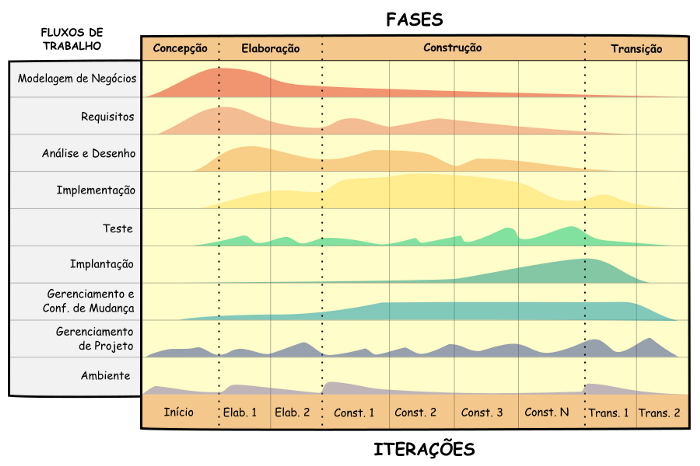
\includegraphics[scale=.5]{rup.png}
    \vspace{5pt}
    \legend{Fonte: \citeonline{DIAS}}
\end{figure}


% \section{Padores de projetop}

% Padrões de projeto
% Os padrões de projeto foram obtidos a partir das ideias apresentadas por Christopher Alexander (ALEXANDER
% et al., 1977), que sugeriu haver padrões comuns de projeto de prédios que eram inerentemente agradáveis e
% eficazes. O padrão é uma descrição do problema e da essência de sua solução, de modo que a solução possa ser
% reusada em diferentes contextos. O padrão não é uma especificação detalhada. Em vez disso, você pode pensar
% nele como uma descrição de conhecimento e experiência, uma solução já aprovada para um problema comum.
% Uma citação do site da Hillside Group (<http://hillside.net:>), dedicado a manter informações sobre os padrões,
% sintetiza seu papel no reúso:
% Padrões e Linguagens de Padrões são formas de descrever as melhores práticas, bons projetos e capturar a experiência
% de uma forma que torne possível a outros reusaressa experiência.
% Os padrões tiveram um enorme impacto no projeto de \textit{software} orientado a objetos. Além de serem soluções
% já testadas para problemas comuns, tornaram-se um vocabulário para falar sobre um projeto. Você pode, portanto,
% explicar seu projeto por meio de descrições dos padrões que você usou. Isso é particularmente verdadeiro para os
% padrões de projeto mais conhecidos que foram originalmente descritos pela 'Gangue dos Quatro'em seu livro de
% padrões (GAMMA et al., 1995). Outras descrições de padrões particularmente importantes são as publicadas em
% uma série de livros de autores da Siemens, uma grande empresa europeia de tecnologia (BUSCHMANN et al., 1996;.
% BUSCHMANN et al., 2007a; BUSCHMANN et al., 2007b; KIRCHER e JAIN, 2004; SCHMIDT et al., 2000).
% Os padrões de projeto são normalmente associados com projeto orientado a objetos. Muitas vezes, os padrões
% publicados contam com as características de objetos, como herança e polimorfismo para fornecer generalidade.
% No entanto, o princípio geral de encapsular a experiência em um padrão é aquele igualmente aplicável a qualquer
% tipo de projeto de \textit{software}. Então, você poderia ter padrões de configuração para os sistemas COTS. Os padrões
% são uma maneira de reusar o conhecimento e a experiência de outros projetistas.
% Os quatro elementos essenciais dos padrões de projeto foram definidos pela 'Gangue dos Quatro', em seu livro
% de padrões:
% 1. Um nome que seja uma referência significativa para o padrão.
% 2. Uma descrição da área de problema que explique quando o modelo pode ser aplicado.
% 3. A descrição da solução das partes da solução de projeto, seus relacionamentos e suas responsabilidades. Essa
% não é uma descrição do projeto concreto; é um modelo para uma solução de projeto que pode ser instanciado
% de diferentes maneiras. Costuma ser expresso graficamente e mostra os relacionamentos entre os objetos e

\section{Aplicação web}
Uma aplicação web envolve diversas camadas da programação, lidando desde a interação com o usuário por meio da interface gráfica com o \textit{frontend}, passando pela manipulação dos dados com o \textit{backend} e o seu armazenamento no banco de dados. Isto, deve ser precedido de um planejamento, explicado na seção \ref{engsoft}.

\subsection{\textit{frontend}}
O \textit{frontend} lida com a interface gráfica e apresentação dos dados ao usuário, ou seja, é onde inclui todo o design, estrutura, layout e o conteúdo das páginas que serão exibidas. O \textit{client-side} deve conter boas práticas de User-Interface
\footnote{É mais uma das ferramentas utilizadas para entregar a boa experiência ao usuário, pois é a parte tangível de um projeto, onde você constrói visualmente o site ou qualquer outra plataforma.}
e User-Experience
\footnote{É tudo que envolve o modo como qualquer usuário interage com o mundo ao seu redor. Na verdade, o termo \textit{user experience}(UX) é muito amplo, mas quando falamos de marcas, produtos, sistemas e serviços, é importante entender que UX não envolve apenas o design do produto e seu desenvolvimento. Temos que observar todas as etapas do cliente junto à sua marca, desde o primeiro “encontro” até o pós-uso ou consumo.} 
para que o conteúdo seja disposto e interpretado pelo usuário da aplicação. \cite{SOUTO}

\subsubsection{Design responsivo}
A união de técnicas de \textit{grids} e imagens fluidos, que se adaptam a proporção da tela que está sendo utilizada faz que o design responsivo se torne uma boa prática no desenvolvimento do \textit{frontend}. A adaptação pode ser apenas o enquadramento de recursos, dada as proporções de altura e largura de uma tela, assim como a reestruturação do layout de forma que os conteúdos sejam exibidos de maneiras distintas nos mais diferentes dispositivos por meio do \textit{media query}. \cite{MOZILA}

\subsubsection{Programação reativa}
A programação reativa é um paradigma que utilizada de chamadas assíncronas para lidar com atualizações em conteúdos estáticos. Fornece um meio eficiente para atualizações de conteúdos utilizando gatilhos como referência \cite{NOLLE}. Segundo \citeonline{NOLLE}, há três formas de ativar o gatilho:
\begin{itemize}
    \item \textbf{Evento}: O evento refere-se a uma situação específica que ocorre via chamadas de \textit{software}.
    \item \textbf{Chamada}: quando faz parte do fluxo da aplicação.
    \item \textbf{Mensagem}: unidade de informação que o sistema envia de volta ao usuário ou operador do sistema com informações sobre o status de uma operação, um erro, falha ou outra condição.
\end{itemize}

Ao digitar em um campo de texto e o que foi escrito ser exibido, com suas edições, na interface da aplicação é um exemplo de programação reativa.

\subsubsection{Interface e experiência do usuário}
A experiência do usuário é o processo para criar produtos que forneçam experiências significativas e relevantes aos usuários \cite{UX}. De acordo com \citeonline{NORMAN}, a definição de usabilidade é um atributo de qualidade na interface ao usuário, que seja eficiente de usar e agradável, sendo a experiência deste ainda mais ampla. 

A experiência do usuário exemplar é atender as necessidades exatas de quem o utiliza, sem quaisquer complicações ou incômodos, podendo ir além com ofertas de simplicidade e elegância, que trazem alegria ao serem vistos e utilizados \cite{NORMAN}. 

% \begin{quote}
%     \aspas{Nenhum produto é uma ilha. Um produto é mais do que o produto. É um conjunto coeso e integrado de experiências. Pense em todas as etapas de um produto ou serviço – desde as intenções iniciais até as reflexões finais, desde o primeiro uso até a ajuda, serviço e manutenção. Faça com que todos trabalhem juntos perfeitamente.}
% \end{quote}

Com o foco no usuário, o produto deve atender as necessidades dele, incluindo sua forma de interação com o sistema, no caso a interface gráfica. Segundo \citeonline{SEBRAEUX}, algumas das métricas para avaliar a experiência do usuário são: usabilidade, taxa de sucesso e taxa de erros.

% https://www.interaction-design.org/literature/topics/ux-design (UX)
% https://bibliotecas.sebrae.com.br/chronus/ARQUIVOS_CHRONUS/bds/bds.nsf/6f47c91e556bb2f56e3ab1eb06a26d3a/$File/30717.pdf (SEBRAE UX)

\subsection{\textit{Backend}}
Segundo a \citeonline{TOTVS}, a função do \textit{backend} está relacionada com banco de dados, servidores, estrutura, gerenciamento de conteúdo e segurança. Podendo ser utilizado para o gerenciamento de login, nesta camada provém a proteção e segurança dos dados armazenados e no tráfego das informações da API. Os usuários não interagem diretamente com o \textit{backend}, necessitando de interfaces para realizar tal manipulação \cite{SOUTO}. A escalabilidade e disponibilidade do sistema dependem desta camada, devido à sua gestão das informações contidas nela, sendo que estas podem estar disponíveis mundialmente.

\subsubsection{API}
A API é um conjunto de rotinas e padrões criados por uma aplicação visando a interoperabilidade entre aplicações. Podendo ser feita na camada de \textit{backend}, uma API requere uma funcionalidade requisitada por um usuário no \textit{frontend} para o \textit{backend} processar os dados e os entregar seguindo um padrão por meio do protocolo HTTP\footnote{Protocolo cliente-servidor que permite obtenção de recursos, como arquivos JSON ou documentos HTML. É a base da troca de dados pelas aplicações \textit{web} que suas mensagens são enviadas por meio de requisições e tem como retorno uma resposta \cite{HTTP}.} \cite{BEECODE}.

\subsection{Framework}
Um framework é um conjunto de ferramentas de programação que fornece funcionalidades genéricas que podem ser alteradas conforme o uso específico. Fornecendo um padrão, é possível criar aplicações reunindo estruturas, bibliotecas de código e seu conjunto de ferramentas documentados que estão prontos para o uso do desenvolvedor.

\subsection{Banco de dados relacional}
Segundo \citeonline{HEUSER}, um banco de dados relacional é composto por tabelas e relações. As tabelas são um conjunto não ordenado de tuplas, que possuem campos com suas propriedades. As relações ligam as tabelas entre si por meio de suas chaves.

\section{Versionamento}
De acordo com a \citeonline{IPSENSE}, o versionamento é uma metodologia aplicada por programadores visando controlar e acompanhar o histórico de alterações em um \textit{software}, permitindo diferenciar mudanças realizadas em cada versão. A manutenção do código, ou seja, adicionar ou alterar informações do sistema para atender novas demandas, pode ser realizada através destas ramificações, diferentes instâncias de um mesmo programa, podendo uma instância conter determinadas alterações enquanto a outra se mantém estável sem as modificações \cite{SOMOSTERA}.